\documentclass{beamer}
\usetheme{Warsaw}  %% Themenwahl

\usepackage[utf8]{inputenc}
\usepackage[ngerman]{babel}
\usepackage{ngerman}
\usepackage{wrapfig}
\usepackage{multicol}
\usepackage{color}

\graphicspath{{../}}
%\pdfimageresolution=300
 
\title[Analyse von SHA256 mit Hilfe von CryptoMiniSat]{Vorstellung der Masterarbeit:\newline Analyse von SHA256 mit Hilfe von CryptoMiniSat}
\author{Lars Schmertmann}
\date{\today\newline\newline\newline Betreuung durch die AG Rechnerarchitektur:\newline Dr. Stephan Eggersglüß und Dr. Daniel Große}
 
\begin{document}
\maketitle
%\setcounter{tocdepth}{3}
%\frame{\tableofcontents}
%\frame{\tableofcontents[currentsection]}

\frame{ \begin{multicols}{2} \tableofcontents \end{multicols} }

\section{Motivation}
  \begin{frame}{Motivation}
    \begin{itemize}
      \setlength{\itemsep}{20pt}
      \item Spaß an der Arbeit mit SAT-Solvern
      \item Spekulationsverlust bei LiteCoin
      \item Masterarbeit zum Thema SHA1/SAT-Solver
      \begin{itemize}
        \item Universität Oslo - Vegard Nossum - November 2012
      \end{itemize}
      \item GitHub-Projekt: SatCoin - (CBMC)
    \end{itemize}
  \end{frame}
\section{Grundlagen}
  \begin{frame}{}
    \begin{center}
      \Huge Grundlagen
    \end{center}
  \end{frame}
  \subsection{Hasheigenschaften}
    \begin{frame}{Hasheigenschaften}
      Ein guter kryptographischer Hash ist:\\
      ~\\
      \begin{itemize}
        \setlength{\itemsep}{20pt}
        \item Kollisionsresistent:
        \begin{itemize}
          \item schwer, $ x \neq y $ zu finden mit $ h(x) = h(y) $
        \end{itemize}
        \item Urbildresistent:
        \begin{itemize}
          \item schwer, zu einem $ a $ ein $ y $ zu finden mit $ a = h(y) $
        \end{itemize}
      \end{itemize}
      ~\\
      Gelingt es die Urbildresistenz zu umgehen,\\
      ist die Kollisionsresistenz ebenfalls umgangen.
    \end{frame}
\subsection{SHA256}
    \begin{frame}{SHA256 / Eckdaten}
      \begin{columns}[T]
        \column{.48\textwidth}
        \begin{itemize}
          \item Nachfolger von SHA-1\\
          \item Standardisierung durch\newline das NIST in 2001\\
          \item Arbeitet in 512 Bit Blöcken\\
          \item Erzeugt einen 256 Bit Hash\\
          \item Besteht aus:\\
          \begin{itemize}
            \item Padding\\
            \item Konstanten\\
            \item Erweiterung\\
            \item Berechnung
          \end{itemize}
        \end{itemize}
        \column{.52\textwidth}
        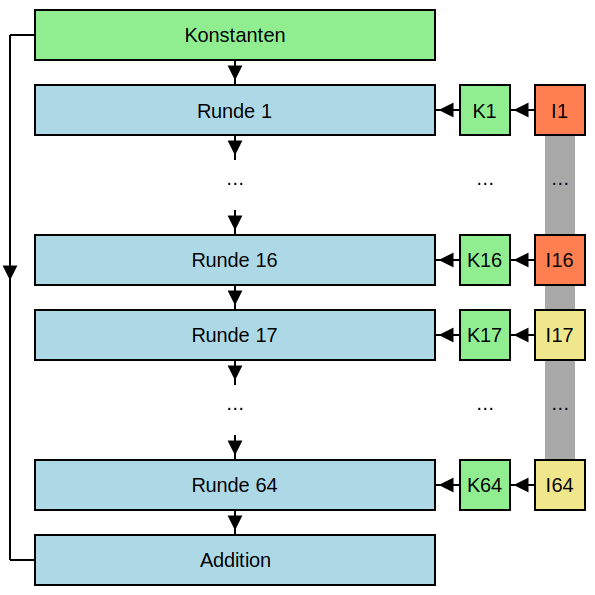
\includegraphics[scale=0.25]{sha256single}
      \end{columns} 
    \end{frame}
    \begin{frame}{SHA256 / Padding}
      Auffüllen der Eingabe auf ein Vielfaches von 512 Bit.\\
      ~\\
      Allgemeines Padding:\\
      ~\\
      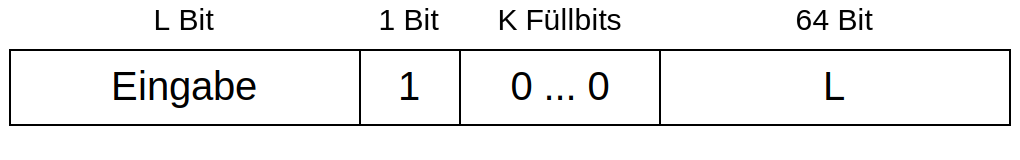
\includegraphics[width=300pt]{padding}\\
    \end{frame}
    \begin{frame}{SHA256 / Funktionen}
      \begin{itemize}
      \setlength{\itemsep}{20pt}
      \item Erweiterung
        \begin{itemize}
          \setlength{\itemsep}{10pt}
          \item $ SSIG0(x) = ROTR^{7}(x)~XOR~ROTR^{18}(x)~XOR~SHR^{3}(x) $
          \item $ SSIG1(x) = ROTR^{17}(x)~XOR~ROTR^{19}(x)~XOR~SHR^{10}(x) $
        \end{itemize}
      \item Berechnung
        \begin{itemize}
          \setlength{\itemsep}{10pt}
          \item $ CH( x, y, z) = (x~AND~y)~XOR~( (NOT~x)~AND~z) $
          \item $ MAJ( x, y, z) = (x~AND~y)~XOR~(x~AND~z)~XOR~(y~AND~z) $
          \item $ BSIG0(x) = ROTR^{2}(x)~XOR~ROTR^{13}(x)~XOR~ROTR^{22}(x) $
          \item $ BSIG1(x) = ROTR^{6}(x)~XOR~ROTR^{11}(x)~XOR~ROTR^{25}(x) $
        \end{itemize}
      \end{itemize}
    \end{frame}
    \begin{frame}{SHA256 / Erweiterung}
      Jeder Block der Länge 512 Bit wird auf 2048 Bit erweitert.\\
      ~\\
      Die zusätzliche Bits werden wie folgt generiert:\\
      ~\\
      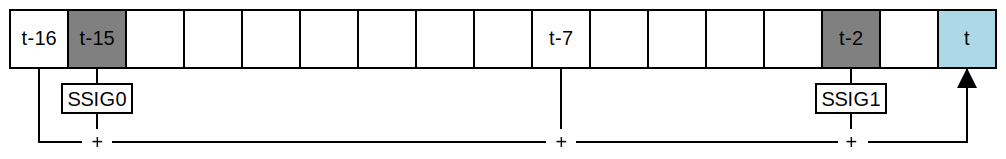
\includegraphics[width=300pt]{extend}
    \end{frame}
    \begin{frame}{SHA256 / Berechnung}
      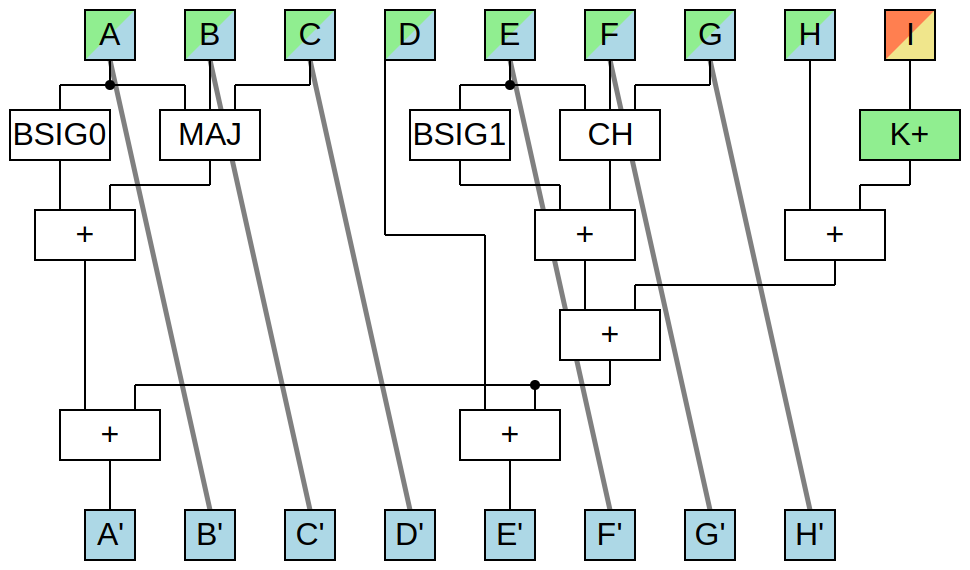
\includegraphics[width=300pt]{sha256core}
    \end{frame}
  \subsection{Bitcoin}
    \begin{frame}
      \frametitle{Bitcoin / Aufgabe}
      Aufbau eines Bitcoinblocks:
      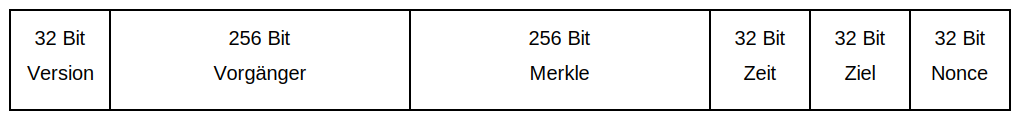
\includegraphics[width=300pt]{bitcoinblock}\\
      ~\\
      Aufgabe:\\
      Finde eine Nonce, so dass SHA256(SHA256(Block))\\
      kleiner als das aktuelle Ziel ist.\\
      ~\\
      Das bedeutet aktuell:\\
      Der Hashwert muss 67 führende Nullen haben.
    \end{frame}
    \begin{frame}{Bitcoin / Padding}
      Eingabe für die erste Hashberechnung:
      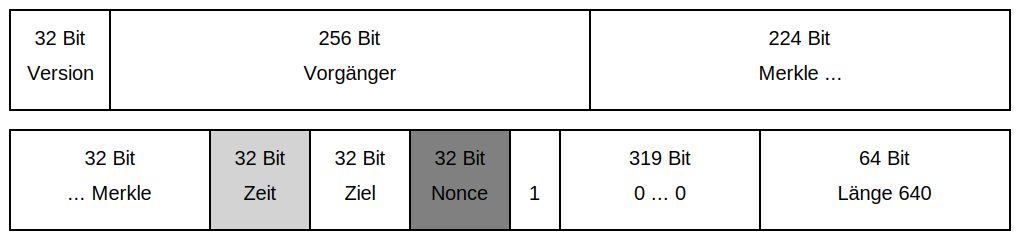
\includegraphics[width=300pt]{blockpadding}\\
      ~\\
      Eingabe für die zweite Hashberechnung:
      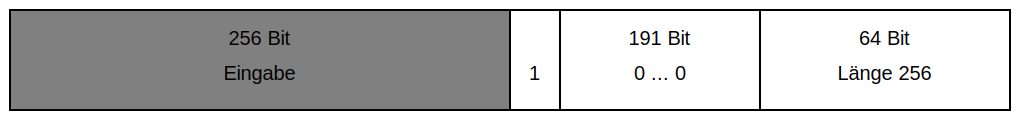
\includegraphics[width=300pt]{blockpadding2}\\
  \end{frame}
  \subsection{CryptoMiniSat / Konjunktive Normalform}
    \begin{frame}{Sat-Solver}
      \begin{itemize}
        \setlength{\itemsep}{20pt}
        \item Versucht zu ermitteln, ob eine aussagenlogische Formel erfüllbar ist
        \item Lösbar in exponentieller Zeit bezüglich der Anzahl Variablen
        \begin{itemize}
          \item NP vollständig
        \end{itemize}
        \item Falls erfüllbar, liefert der SAT-Solver ein Beispiel
        \item Enthält u.a. Heuristiken und Lernverfahren
        \item Transformation von SHA256 in ein Erfüllbarkeitsproblem
        \begin{itemize}
         \item In diesem Fall die konjunktive Normalform
        \end{itemize}
      \end{itemize}
    \end{frame}
    \begin{frame}{Konjunktive Normalform}
      \begin{itemize}
        \setlength{\itemsep}{16pt}
        \item Eine Formel der Aussagenlogik ist in konjunktiver Normalform, wenn sie eine Konjunktion von Disjunktionstermen ist
        \item Literal: nichtnegierte oder negierte Variable
        \item Klausel: ein Disjunktionsterm
        \item Eine Formel in KNF hat also die Form: \newline \newline $ \bigwedge\limits_{i} \bigvee\limits_{j} (\neg)x_{ij} $
        \item Beispiel: $ (\neg a \vee \neg b \vee \neg c) \wedge (\neg a \vee b \vee c) $
      \end{itemize}
    \end{frame}
    \begin{frame}{Tseitin-Transformation}
      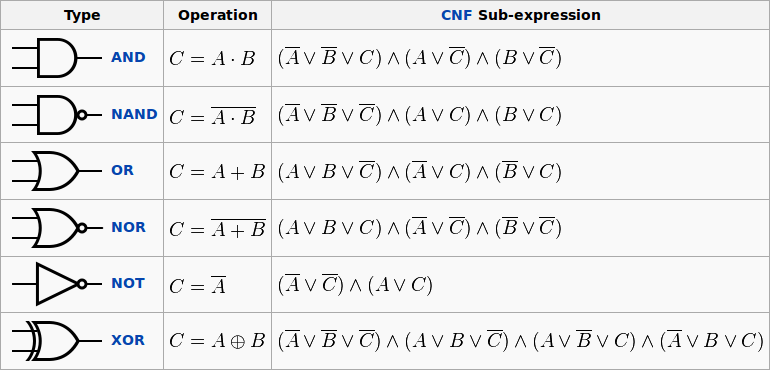
\includegraphics[scale=1]{tseitin.png}\\
      Quelle: https://en.wikipedia.org/wiki/Tseitin\_transformation
    \end{frame}
    \begin{frame}{Espresso}
      Heuristic Logic Minimizer der Berkeley Universität von 1989\\
      ~\\
      Am Beispiel von AND:\\
      ~\\
      \begin{tabular}{ccc|cp{1cm}ccc|cp{1cm}l}
        a & b & r & c & & a & b & r & c\\
        \cline{1-4}\cline{6-9}
        1 & 1 & 0 & 0 & & 1 & 1 & 0 & 0 & & $ (\neg a \vee \neg b \vee c) $\\
        1 & 0 & 1 & 0 & & X & 0 & 1 & 0 & & $ (b \vee \neg c) $\\
        0 & 1 & 1 & 0 & & 0 & X & 1 & 0 & & $ (a \vee \neg c) $\\
        0 & 0 & 1 & 0 \\
        \cline{1-4}
        1 & 1 & 1 & 1 \\
        1 & 0 & 0 & 1 \\
        0 & 1 & 0 & 1 \\
        0 & 0 & 0 & 1 \\
      \end{tabular}
    \end{frame}
    \begin{frame}{XOR}
      Die Klauselmenge für ein XOR wächst exponentiell. Beispiel:\\
      ~\\
      $n = 2$:~~~~$ a \Leftrightarrow b \veebar c$\\
      ~\\
      4 Klauseln mit jeweils 3 Literalen
      ~\\
      $ (\neg a \vee \neg b \vee \neg c) \wedge (\neg a \vee b \vee c) \wedge (a \vee \neg b \vee c) \wedge (a \vee b \vee \neg c) $\\
      ~\\
      Allgemein: $ 2^{n - 1} $ Klauseln mit jeweils $ n $ Literalen\\
      ~\\
      CryptoMiniSat akzeptiert auch XOR-Klauseln: $ (\neg a \veebar b \veebar c)$\\
    \end{frame}

\section{Umsetzung}
  \begin{frame}{}
    \begin{center}
      \Huge Umsetzung
    \end{center}
  \end{frame}
  \subsection{Padding}
    \begin{frame}{Padding}
      Mögliche Lösung für SAT-Berechnung\\
      \begin{itemize}
       \item Länge von 55 Byte vorgeben:
      \end{itemize}
      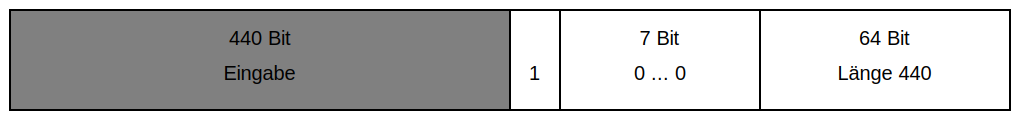
\includegraphics[width=300pt]{padding-allgemein}
    \end{frame}
  \subsection{Funktionen}
    \begin{frame}{CH}
      $ CH( x, y, z) = (x~AND~y)~XOR~( (NOT~x)~AND~z) $\\
      ~\\
      $ c \Leftrightarrow (x \wedge y) \veebar ( \neg x \wedge z) $\\
      ~\\
      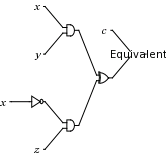
\includegraphics[scale=0.5]{ch.png}\\
      ~\\
      $ (\neg c \vee \neg x \vee y) \wedge (\neg c \vee x \vee z) \wedge (c \vee \neg x \vee \neg y) \wedge (c \vee x \vee \neg z) $
    \end{frame}
    \begin{frame}{MAJ}
      $ MAJ( x, y, z) = (x~AND~y)~XOR~(x~AND~z)~XOR~(y~AND~z) $\\
      ~\\
      $ m \Leftrightarrow (x \wedge y) \veebar (x \wedge z) \veebar (y \wedge z) $\\
      ~\\
      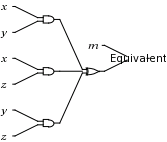
\includegraphics[scale=0.5]{maj.png}\\
      ~\\
      $ (\neg m \vee x \vee y) \wedge  (\neg m \vee x \vee z) \wedge (\neg m \vee y \vee z) \wedge $\\
      $ (m \vee \neg x \vee \neg y) \wedge (m \vee \neg x \vee \neg z) \wedge (m \vee \neg y \vee \neg z) $
      \end{frame}
    \begin{frame}{*SIG*}
      $ *SIG*(a, b, c) = a~XOR~b~XOR~c $\\
      ~\\
      $ s \Leftrightarrow a \veebar b \veebar c $\\
      ~\\      
      \begin{columns}[C]
        \column{.4\textwidth}
        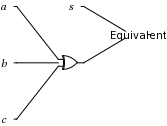
\includegraphics[scale=0.5]{sig.png}
        \column{.5\textwidth}
        $ \Rightarrow (\neg s \veebar a \veebar b \veebar c) $
      \end{columns}
      ~\\
      ~\\
      $ (\neg a \vee \neg b \vee \neg c \vee s) \wedge (\neg a \vee \neg b \vee c \vee \neg s) \wedge (\neg a \vee b \vee \neg c \vee \neg s) \wedge$\\
      $ (\neg a \vee b \vee c \vee s) \wedge (a \vee \neg b \vee \neg c \vee \neg s) \wedge (a \vee \neg b \vee c \vee s) \wedge $\\
      $ (a \vee b \vee \neg c \vee s) \wedge (a \vee b \vee c \vee \neg s) $
    \end{frame}
    \begin{frame}{Carry-Riple-Addierer}
      32 Bit Addierer : 1 Halbaddierer + 30 Volladdierer + 1 XOR\\
      ~\\
      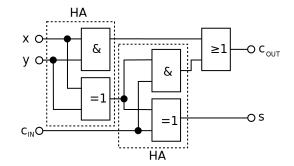
\includegraphics[scale=0.5]{volladdierer}\\
      $ (c_{out} \vee \neg x \vee \neg y) \wedge (\neg c_{out} \vee x \vee y) \wedge (c_{out} \vee \neg x \vee \neg c_{in}) \wedge $\\
      $ (c_{out} \vee \neg y \vee \neg c_{in}) \wedge (\neg c_{out} \vee x \vee c_{in}) \wedge (\neg c_{out} \vee y \vee c_{in}) $\\
      ~\\
      $ (\neg s \veebar x \veebar y \veebar c_{in})$\\
    \end{frame}
  \subsection{Komposition}
  \begin{frame}{CBMC vs Eigenbau}
    \begin{itemize}
      \item CBMC
      \begin{itemize}
        \item $ \sim $ 70.000 Variablen
        \item $ \sim $ 350.000 Klauseln
      \end{itemize}
      \item Eigenbau
      \begin{itemize}
        \item $ \sim $ 50.000 Variablen
        \item $ \sim $ 250.000 Klauseln
      \end{itemize}
      \item Eigenbau mit XOR
      \begin{itemize}
        \item $ \sim $ 50.000 Variablen
        \item $ \sim $ 150.000 Klauseln
      \end{itemize}
    \end{itemize}
  \end{frame}

\section{Ergebnisse}
  \begin{frame}{}
    \begin{center}
      \Huge Ergebnisse
    \end{center}
  \end{frame}
  \subsection{Allgemein}
    \begin{frame}{Kern}
      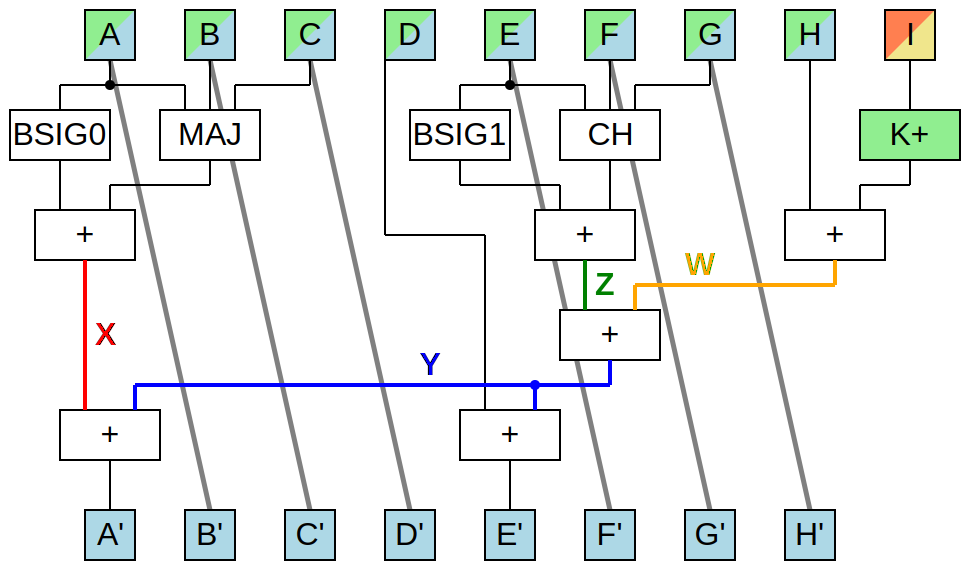
\includegraphics[width=300pt]{sha256coreA}\\
      D = E' + \textcolor{blue}{\textbf{X}} - A'\\
      %\pause
      %~~~~~~~~~~~~~~~~~~~~~~ $ \Rightarrow $ D = E' + (\textcolor{blue}{\textbf{X}} - A')~~~~~~ $ \Rightarrow $ D = A' - (\textcolor{blue}{\textbf{X}} - A')\\
      %~~~~~~~~~~~~~~~~~~~~~~ $ \Rightarrow $ D = A' - \textcolor{blue}{\textbf{X}} + A'~~~~~~~~ $ \Rightarrow $ D = 2 $\cdot$ A' - \textcolor{blue}{\textbf{X}}
    \end{frame}
  \subsection{Sat-Solving 1 - Einzelner Lösungsversuch}
    \begin{frame}{Einzelne Lösungsversuche}
      \begin{itemize}
        \setlength{\itemsep}{20pt}
        \item Vorwärtsberechnung funktioniert
        \pause
        \item Rückwärtsberechnung funktioniert nicht
        \pause
        \item Rückwärtsberechnung funktioniert mit Runden 1 - 18
        \pause
        \item Rückwärtsberechnung ohne Runden 17 - 20 funktioniert
        \pause
        \item Rückwärtsberechnung ohne Erweiterung 17 - 24 funktioniert
      \end{itemize}
    \end{frame}
  \subsection{Sat-Solving 2 - Iterative Lösungsversuche}
    \begin{frame}{Iterative Lösungsversuche}
      \begin{itemize}
        \setlength{\itemsep}{20pt}
        \item Rückwärtsbrechnung funktioniert mit bis zu 19 Bits
        \pause
        \item Rückwärtsberechnung mit 1,3 Gigabyte Konfliktklauseln:\\ Funktioniert mit bis zu 23 Bits
        \pause
        $ \Rightarrow $ Zusätzliche Klauseln begrenzen den Lösungsraum und helfen dem SAT-Solver
        \pause
        \item $ \Rightarrow $ Konfliktklausel-Mining
      \end{itemize}
    \end{frame}
    \begin{frame}{Konfliktklausel-Mining}
      \begin{itemize}
       \item Konfliktklausel ausdenken und Literale einzeln negiert in die SAT-Instanz einfügen:\\Falls nicht lösbar ist die Konfliktklausel gültig
       \pause
       \item Scheitert an den Komplexität.\\Beispiel für Klauseln mit 2 Literalen:
       \item Bei 50.000 Literalen ergeben sich\\ 50.000 $ \cdot $ 49.999 = 2.499.950.000 Kombinationen
       \item Klauseln mit 2 Literalen können 4 Belegungen abbilden:\\ 2.499.950.000 $ \cdot $ = 9.999.800.000 Klauseln
      \end{itemize}
    \end{frame}
  \subsection{Sat-Solving 3 - Analyse der Konfliktklauseln}
    \begin{frame}{Analyse der Konfliktklauseln}
      \begin{enumerate}
        \setlength{\itemsep}{20pt}
        \item Entfernen schon bekannter Klauseln
        \item Identifizierung und Normalisierung modulspezifischer Klauseln
        \pause
        \item Bewertung der modulübergreifenden Klauseln:
        \begin{itemize}
          \item SHA256 als ungerichter Graph mit ca. 1000 Knoten
          \item Berechnung der Distanz der Knoten zueinander mit Dijkstra
          \item Klauselbewertung ergibt sich durch: max\_dist - module + 1
        \end{itemize}
      \end{enumerate}
    \end{frame}
    \begin{frame}{Weitere Konfliktklauseln testen}
      \begin{itemize}
        \setlength{\itemsep}{20pt}
        \item "`Wertvolle"' Klauseln übertragen auf:
        \begin{itemize}
          \item Vorhergehende oder Nachfolgende Runden
          \item Vorhergehende oder Nachfolgende Bits
        \end{itemize}
        \item Bei der Hälfte der Klauseln sehr erfolgreich
      \end{itemize}
      \pause
      ~\\
      Mit 22 Megabyte Klauseln:\\
      Rückwärtsbrechnung funktioniert mit bis zu 25 Bits
    \end{frame}

\begin{frame}{}
  \begin{center}
    \begin{LARGE}
      Vielen Dank für\\
      eure Aufmerksamkeit\\
      ~\\
      
\includegraphics[scale=0.2]{smilie.png}
    \end{LARGE}
  \end{center}
\end{frame}

\begin{frame}{Fragen}
  \begin{center}
    \begin{LARGE}
      \begin{tabular}{ccccc}
         & \textbf{?} & \textbf{?} & \textbf{?} & \\
        \textbf{?} & \textbf{?} &  & \textbf{?} & \textbf{?}\\
         &  &  & \textbf{?} & \textbf{?}\\
         &  & \textbf{?} & \textbf{?} & \\
         & \textbf{?} & \textbf{?} &  & \\
         &  &  &  & \\
         & \textbf{?} & \textbf{?} &  & \\
         & \textbf{?} & \textbf{?} &  & 
      \end{tabular}
    \end{LARGE}
  \end{center}
\end{frame}

\end{document}